\documentclass[12pt]{article}

\include{preamble}
\usepackage{tikz}
\usepackage{dsfont}
\usepackage{xfrac}
\newcommand{\indicator}[1]{\mathds{1}_{#1}}


\newtoggle{professormode}
%\toggletrue{professormode} %STUDENTS: DELETE or COMMENT this line



\title{MATH 390.4 / 650.2 Spring 2018 Homework \#5t}

\author{Darshan Patel} %STUDENTS: write your name here

\iftoggle{professormode}{
\date{Due 11:59PM Friday, May 18, 2018 under the door of KY604 \\ \vspace{0.5cm} \small (this document last updated \today ~at \currenttime)}
}

\renewcommand{\abstractname}{Instructions and Philosophy}

\begin{document}
\maketitle

\iftoggle{professormode}{
\begin{abstract}
The path to success in this class is to do many problems. Unlike other courses, exclusively doing reading(s) will not help. Coming to lecture is akin to watching workout videos; thinking about and solving problems on your own is the actual ``working out.''  Feel free to \qu{work out} with others; \textbf{I want you to work on this in groups.}

Reading is still \textit{required}. For this homework set, read about all the concepts introduced in class online e.g. probabilistic classification, the logistic link function, performance characteristics of binary classification, asymmetric cost / reward classifiers, bias-variance decomposition, bagged models, RandomForests$^\circledR$, correlation, causation, lurking variables and graphical depictions of causal models. It is your responsibility to supplement the notes with your own readings. Also, read the introduction in Finlay.

The problems below are color coded: \ingreen{green} problems are considered \textit{easy} and marked \qu{[easy]}; \inorange{yellow} problems are considered \textit{intermediate} and marked \qu{[harder]}, \inred{red} problems are considered \textit{difficult} and marked \qu{[difficult]} and \inpurple{purple} problems are extra credit. The \textit{easy} problems are intended to be ``giveaways'' if you went to class. Do as much as you can of the others; I expect you to at least attempt the \textit{difficult} problems. 

This homework is worth 100 points but the point distribution will not be determined until after the due date. See syllabus for the policy on late homework.

Up to 10 points are given as a bonus if the homework is typed using \LaTeX. Links to instaling \LaTeX~and program for compiling \LaTeX~is found on the syllabus. You are encouraged to use \url{overleaf.com}. If you are handing in homework this way, read the comments in the code; there are two lines to comment out and you should replace my name with yours and write your section. The easiest way to use overleaf is to copy the raw text from hwxx.tex \emph{and} preamble.tex into two new overleaf tex files with the same name. If you are asked to make drawings, you can take a picture of your handwritten drawing and insert them as figures or leave space using the \qu{$\backslash$vspace} command and draw them in after printing or attach them stapled.

The document is available with spaces for you to write your answers. If not using \LaTeX, print this document and write in your answers. I do not accept homeworks which are \textit{not} on this printout. Keep this first page printed for your records.

\end{abstract}

\thispagestyle{empty}
\vspace{1cm}
NAME: \line(1,0){380}
\clearpage
}


\problem{These are questions about the Finlay's introduction to his book.}

\begin{enumerate}

\easysubproblem{Finlay introduces predictive analytics by using the case study of what supervised learning problem? Explain.}\spc{4} \\
Finlay introduces predictive analytics by using the case study of credit scoring, which we also looked at in the beginning of the semester. Predictive analytics was used to determine if a customer could take out a loan, credit card, mortgage, etc. This was initially done by human underwriters who just made an expert opinion on each application. Now, with predictive models, we are better able to determine credit scoring using FICO scores to determine whether a customer's application should go through or not. 

\hardsubproblem{What does a credit score of 700 mean? Use figure 1.2 on page 5 when answering this question.}\spc{3} \\
A credit score of $700$ means an individual has a $1024$ odds of default. This means that if you have $1025$ borrowers that score $700$, the expectation is that $1024$ will repay what they borrowed and $1$ will not. 


\hardsubproblem{How much more likely is someone to default if that have 9 or more credit cards than someone with 4-8 credit cards?}\spc{3} \\
If someone has $9$ or more credit cards than someone with $4$ to $8$ credit cards, their credit score will fall by $18$ points. Assuming all other variables the same, the one with the credit score of $700$ will default at the odds of $1024:1$ while the one with credit score of $700 - 18 = 682$ will default at the odds of $\approx 800:1$. This means that if you have $801$ borrowers that score $682$, the expectation is that only $800$ will repay what they borrowed. The change is $$ \frac{\frac{1}{801} - \frac{1}{1025}}{\frac{1}{1025}} \approx 28\% $$ 

\newpage
\easysubproblem{Summarize Finlay's conception of \qu{big data}.}\spc{8} \\
Big data has four features: volume, variety, volatility and multi-sourced. Big data deals with any database that is too large to be comfortably managed on an average PC/laptop/server. It contains many different types of structured and unstructured data. Big data also deals with data that is not stable, such as heart rate and address. Some big data sources are generated from one source whereas some are from many different sources which introduces additional issues around data quality, privacy and security. 

\end{enumerate}


\problem{This question is about probability estimation. We limit our discussion to estimating the probability that a single event occurs.}


\begin{enumerate}

\easysubproblem{What is the difference between the regression framework and the probability estimation framework?}\spc{6} \\
The regression framework gives a model a full picture of what an outcome will be. By using the probability estimation framework, it gives the model probabilities of how likely one or more feature will affect a predicted phenomenon. 

\easysubproblem{Is probability estimation more similar to regression or classification and why?}\spc{3} \\
Probability estimation is more similar to classification because it tries to predict whether something is a $1$ or $0$, or success or failure.

\hardsubproblem{Why was it necessary to think of the response $Y$ as a random variable and why in particular the Bernoulli random variable?}\spc{3} \\
It is necessary to think of the response $Y$ as a Bernoulli random variable because a Bernoulli random variable only has $2$ outcomes, $0$ and $1$. The response $Y$ also has two outcomes only. 

\hardsubproblem{If we use the Bernoulli r.v. for $Y$, are there any error terms (i.e. $\delta, \epsilon, e$) anymore? Yes/\fbox{no}.}\spc{0} 

\easysubproblem{What is the difference between $f$ in the regression framework and $f_{pr}$ in the probabilistic classification framework?}\spc{6} \\
The difference between $f$ in the regression framework and $f_{pr}$ in the probabilistic classification framework is that $f$ is a polynomial and $f(\vec{x}) \in \mathbb{R}$ whereas $f_{pr} \in (0,1)$ since it goes into the Bernoulli distribution as a parameter. $f_{pr}$ is the probability $\prob{Y |\vec{x}} = 1$. 


\hardsubproblem{Is there a $t_{pr}$? If so, what does it look like?}\spc{3} \\
There is a $t_{pr}$ and it looks like $g_{pr}$ because we want $f_{pr}$ to be close to $t_{pr}$. 

\newpage
\easysubproblem{Write out the likelihood as a function of $f_{pr}$, the $\x_i$'s and the $y_i$'s.}\spc{3} 
$$ \prob{Y_1,\dots,Y_n} = \prod_{i=1}^n f_{pr}(\x_i)^{y_i}(1-f_{pr}(\x_i))^{1-y_i} $$ 

\hardsubproblem{What assumption did you have to make and what would happen if you didn't make this assumption?}\spc{3} \\
We assumed that there is no dependence structure between $Y_1,\dots,Y_n$. If we don't make this assumption, then $\prob{Y_1,\dots,Y_n}$ is unknown and probably will be messy to get in a canonical form. 

\easysubproblem{Is $f_{pr}$ knowable? Yes/\fbox{no}.}\spc{0}

\end{enumerate}


\problem{This question continues the discussion of probability estimation for one event via the logistic regression approach.}

\begin{enumerate}

\intermediatesubproblem{As before, if we are to get anywhere at all, we need to approximate the true function $f_{pr}$ with a function in a hypothesis set, $\mathcal{H}_{pr}$. Let us examine the range of all elements in $\mathcal{H}_{pr}$. What values can these functions return and why?}\spc{4} \\
These functions can only return values in $(0,1)$ because we want to define a probability for attaining a $1$. 

\hardsubproblem{We would also feel warm and fuzzy inside if the elements of $\mathcal{H}_{pr}$ contained the term $\w \cdot \x$.  What is the main reason we would like our prediction functions to contain this linear component?}\spc{1} \\
Our prediction functions should contain this linear component so if we have a high $\w \cdot \x$, we can return a high probability using the function in $\mathcal{H}_{pr}$. 

\easysubproblem{The problem is $\w \cdot \x \in \reals$ but in (a) there is a special range of allowable functions. We need a way to transform $\w \cdot \x$ into the range from (a). What is this function called?}\spc{0} \\ 
link/activation function.

\easysubproblem{Give some examples of such functions.}\spc{2} 
\begin{itemize} 
\item Logistic function: $\Phi(u) = \frac{e^u}{1 + e^u}$ 
\item Complementary Log-Log function: $\Phi(u) = 1 - e^{-e^u}$ 
\item Hyperbolic Tangent function: $\Phi(u) = \frac{e^u - e^{-u}}{e^u + e^{-u}}$ \end{itemize} 

\easysubproblem{We will choose the logistic function. Write the likelihood again from 2(g) but replace $f_{pr}$ with the element from $\mathcal{H}_{pr}$ that uses the logistic function.}\spc{2}
$$ \prob{Y_1,\dots,Y_n} = \prod_{i=1}^n (\frac{e^{\w \cdot \x}}{1+e^{\w \cdot \x}})^{y_i}(1 - \frac{e^{\w \cdot \x}}{1 + e^{\w \cdot \x}})^{1-y_i} $$ 

\hardsubproblem{Simplify your answer from (e) so that you arrive at:

\beqn
\sum_{i=1}^n \natlog{1 + e^{(1 - 2y_i) \w \cdot \x_i}}
\eeqn}~\spc{10} 

$$\begin{aligned} \b &= \argmax_{\w} \set{\prob{Y_i, \dots,Y_n}} 
\\ &= \argmax_{\w} \set{\prod_{i=1}^n (\frac{e^{\w \cdot \x_i}}{1 + e^{\w \cdot \x_i}})^{y_i}(1 - \frac{e^{\w \cdot \x_i}}{1 + e^{\w\cdot \x_i}})^{1 - y_i}} 
\\ &= \argmax_{\w} \set{ \prod_{i=1}^n (\frac{1}{1 + e^{-\w \cdot \x_i}})^{y_i}(\frac{1}{1+e^{\w \cdot \x_i}})^{1 - y_i}} 
\\ &= \argmax_{\w} \set{ \prod_{i=1}^n \begin{cases} (1 + e^{-\vec{w} \cdot \vec{x}_i})^{-1} &\text{ if } y_i = 1  \\ (1 + e^{\vec{w} \cdot \vec{x}_i})^{-1} &\text{ if } y_i = 0 \end{cases} }
\\ &= \argmax_{\w} \set{\prod_{i=1}^n (1 + e^{(1 - 2y_i)\w \cdot \x_i})^{-1} }
\\ &= \argmax_{\w} \set{ \sum_{i=1}^n \ln(1 + e^{(1-2y_i)\w \cdot \x_i})} \end{aligned} $$ 

\extracreditsubproblem{We will now maximize this likelihood w.r.t to $\w$ to find $\b$, the best fitting solution which will be used within $g_{pr}$ i.e.

\beqn
\b = \argmax_{\w \in \reals^{p+1}}\braces{\sum_{i=1}^n \natlog{1 + e^{(1 - 2y_i) \w \cdot \x_i}}}
\eeqn

to do so, we should find the derivative and set it equal to zero i.e.

\beqn
\derivop{\w}{\sum_{i=1}^n \natlog{1 + e^{(1 - 2y_i) \w \cdot \x_i}}} ~\buildrel \text{set} \over =~ 0
\eeqn

Try to find the derivative and solve. Get as far as you can. Do so on a separate page}\spc{0} \\ See page $12$. 

\easysubproblem{If you attempted the last problem, you found that there is no closed form solution. What type of methods are used to approximate $\b$? Note: once you use such methods and arrive at a $\b$, that is called \qu{running a logistic regression}. }\spc{1} \\ To approximate $\b$, use numerical methods such as gradient descent (or my favorite, stochastic gradient descent). 

\easysubproblem{In class we used the notation $\phat = g_{pr}$. Why?}\spc{1} \\
We want to find the probability of attaining a $1$ in our model using $\x$ and so we let that equal $g_{pr}$. 

\easysubproblem{Write down $\phat$ as a function of $\b$ and $\x$.}\spc{2}
$$ \phat = (1 + e^{-\b \cdot \x})^{-1} $$ 

\intermediatesubproblem{What is the interpretation of the linear component $\b \cdot \x$? What does it mean for $\phat$? No need to give the full, careful interpretation.}\spc{4} \\
The interpretation of the linear component is $\ln (\frac{\phat}{1-\phat})$. This is the log-odds of $Y$ given $\x$. The more positive and larger the log odds is, the higher the probability is. 

\hardsubproblem{How does one go about \textit{validating} a logistic regression model? What is the fundamental problem with doing so that you didn't have to face with regression or classification? Discuss.}\spc{4} \\
To validate a logistic regression model, validate against $f_{pr}$; but this is not possible and so we have to validate $\phat$ versus $\y$. This is different from validation in regression and classification because we are not directly comparing our model to $f_{pr}$, but rather just looking at probabilities. $\y$ is in $\mathbb{R}$ whereas $\phat$ is in $(0,1)$. We have to turn a $\phat$ into a $\yhat$ using probability estimation to do classification. 

\end{enumerate}


\problem{This question is about probabilistic classification i.e. using probability estimation to classify. We limit our discussion to binary classification.}


\begin{enumerate}

\easysubproblem{How do you use a probability estimation model to classify. Provide the formula which provides $\hat{y}(\phat)$ i.e. the estimate of whether the event of interest occurs as a function of the probability estimate of the event occurring. Use the \qu{default} rule.}\spc{1}  $$ \hat{y}_i = \indicator{\hat{p}_i \geq 0.5} $$ 

\easysubproblem{In the formula from (a), there is an option to be made, write the formula again below with this option denoted $p_{th}$.}\spc{1}
$$ \hat{y}_i = \indicator{\hat{p}_i \geq p_{th}}$$ 

\intermediatesubproblem{What happens when $p_{th}$ is low and what happens when $p_{th}$ is high? What is the tradeoff being made?}\spc{4} \\
When $p_{th}$ is low, there are more false positives and less false negatives because it is easier to get a $1$ than a $0$. On the other hand, when $p_{th}$ is high, there are less false positives and more false negatives because it is harder to get a $1$ than a $0$. The tradeoff being made is between how many false positive and false negatives you have. 

\hardsubproblem{Below is the first 20 rows of in-sample prediction results from a logistic regression whose reponse is $>50K$ (the positive class) or $\leq 50K$ (the negative class). You have the $\phat_i$'s and the $y_i$'s. Create a performance table that includes the four numbers in the confusion table as well as FPR and recall. Leave some room for one additional column we will compute later in the question. The rows in the table should be indexed by $p_{th} \in \braces{0, 0.2, \ldots, 0.8, 1}$ which you should use as the first column. Hint: you may want to sort by $\phat$ and convert $y$ to binary before you begin. }

$$ \begin{tabular}{|c|c|c|c|c|c|c|c|c|}
  \hline
$\phat$ & $y$ & $y$ & $\indicator{\phat \geq 0.0}$ & $\indicator{\phat \geq 0.2}$ & $\indicator{\phat \geq 0.4}$ & $\indicator{\phat \geq 0.6}$ & $\indicator{\phat \geq 0.8}$ & $\indicator{\phat \geq 1.0}$ \\ 
  \hline
  0.00 & $<$=50K & 0 & 1 & 0 & 0 & 0 & 0 & 0 \\ 
  0.00 & $<$=50K & 0 & 1 & 0 & 0 & 0 & 0 & 0 \\ 
  0.01 & $<$=50K & 0 & 1 & 0 & 0 & 0 & 0 & 0 \\  
  0.01 & $<$=50K & 0 & 1 & 0 & 0 & 0 & 0 & 0 \\ 
  0.01 & $<$=50K & 0 & 1 & 0 & 0 & 0 & 0 & 0 \\ 
  0.02 & $<$=50K & 0 & 1 & 0 & 0 & 0 & 0 & 0  \\ 
  0.07 & $<$=50K & 0 & 1 & 0 & 0 & 0 & 0 & 0 \\
  0.07 & $<$=50K & 0 & 1 & 0 & 0 & 0 & 0 & 0 \\
  0.07 & $>$50K & 1 & 1 & 0 & 0 & 0 & 0 & 0 \\ 
  0.08 & $<$=50K & 0 & 1 & 0 & 0 & 0 & 0 & 0 \\
  0.32 & $<$=50K & 0 & 1 & 1 & 0 & 0 & 0 & 0 \\ 
  0.35 & $>$50K & 1 & 1 & 1 & 0 & 0 & 0 & 0  \\ 
  0.35 & $>$50K & 1 & 1 & 1 & 0 & 0 & 0 & 0 \\ 
  0.38 & $<$=50K & 0 & 1 & 1 & 0 & 0 & 0 & 0 \\ 
  0.49 & $>$50K & 1 & 1 & 1 & 1 & 0 & 0 & 0 \\ 
  0.59 & $>$50K & 1 & 1 & 1 & 1 & 0 & 0 & 0 \\ 
  0.69 & $>$50K & 1 & 1 & 1 & 1 & 1 & 0 & 0 \\ 
  0.73 & $>$50K & 1 & 1 & 1 & 1 & 1 & 0 & 0 \\ 
  0.76 & $>$50K & 1 & 1 & 1 & 1& 1 & 0 & 0 \\ 
  0.91 & $>$50K & 1 & 1 & 1 & 1 & 1 & 1 & 0 \\ \hline
\end{tabular} $$ 

$$ 
 \begin{tabular}{|c|cccc|cccc|} \hline 
$p_{th}$ & TP & TN & FP & FN & FPR & Recall & FDR & FNR \\ \hline 
0.0 & 9 & 0 & 11 & 0 &
 $\sfrac{11}{11}$ & $\sfrac{9}{9}$ & \sfrac{11}{20} & $\sfrac{0}{9}$  \\ \hline 
0.2 & 8 & 9 & 2 & 1 &
 $\sfrac{2}{11}$ & $\sfrac{8}{9}$ & $\sfrac{2}{10}$ & $\sfrac{1}{9}$ \\ \hline
0.4 & 6 & 11 & 0 & 3 &
 $\sfrac{0}{11}$ & $\sfrac{6}{9}$ & $\sfrac{0}{6}$ & $\sfrac{3}{9}$ \\ \hline 
0.6 & 4 & 11 & 0 & 5 &
 $\sfrac{0}{11}$ & $\sfrac{4}{9}$ & $\sfrac{0}{4}$ & $\sfrac{5}{9}$ \\ \hline 
0.8 & 1 & 11 & 0 & 8 &
 $\sfrac{0}{11}$ & $\sfrac{1}{9}$ & $\sfrac{0}{1}$ & $\sfrac{8}{9}$ \\ \hline 
1.0 & 0 & 11 & 0 & 9 &
 $\sfrac{0}{11}$ & $\sfrac{0}{9}$ & $\sfrac{0}{0}$ & $\sfrac{9}{9}$ \\ \hline 
\end{tabular} $$

\newpage
\intermediatesubproblem{Using the performance table from (d), trace out an approximate ROC curve.}\spc{6}
$$ \includegraphics[width = 10.0cm]{ROC} $$ 

\intermediatesubproblem{Using the performance table from (d), trace out an approximate DET curve.}\spc{6}
$$ \includegraphics[width = 10.0cm]{DET} $$ 

\easysubproblem{Consider the $c_{FP} = \$5$ and $c_{FN} = \$1,000$. Explain how you would find the probabilistic classifier model that minimizes cost among the $p_{th}$ values you considered in your performance table in (d) but do not do any computations.}\spc{6} \\
To minimize costs, you want to minimize FN because since the cost of getting a false negative is $\$1,000$. To do this, keep $p_{th}$ small. Create probabilistic classifier models using small $p_{th}$ on $\mathcal{D}_{\text{train}}$ and then test it on $\mathcal{D}_{\text{test}}$. Determine which $p_{th}$ creates the biggest average reward and use that $p_{th}$. 

\end{enumerate}


\problem{These are questions related to bias-variance decomposition, bagging and random forests. }

\begin{enumerate}

\easysubproblem{List the assumptions for the bias-variance decomposition.}\spc{3} \\
Assume that $\expe{Y  ~|~ \X = \x}  =f(\x)$, or $ \expe{\Delta ~|~ \X = \x} = 0$ where $\Delta$ is the random variable for error. Also assume that the variance does not depend on $\x$, meaning $\var{\Delta ~|~ \X = \x} = \var{\Delta} = \sigma^2$ and so $\expe{\Delta^2} = 0$. 


\intermediatesubproblem{Why is $f(\x)$ called the \qu{conditional expectation function}?}\spc{3} \\
$f(\x)$ is called the conditional expectation function because it is the expected value of $Y$ given $\X = \x$, or $\expe{Y ~|~ \X = \x}$. 


\easysubproblem{Provide an expression for the bias-variance decomposition formula for the average MSE over the distribution $\prob{\X}$ for $y = g + (f-g) + \delta$. You should have three terms in the expression. Make sure you explain conceptually each term in English.}\spc{3} 
$$ \text{MSE} = \sigma^2 + \mathrm{E}_{\X}[\var{g(\x)}] + \mathrm{E}_{\X}[\text{Bias}[g(\x)]^2] $$ where $\sigma^2$ is the variance of $Y$, the middle term explains how much $g$ varies around its mean function $\expe{g(\x)}$ and the last term explains how far away the average $g$ is from $f$. 

\extracreditsubproblem{Rederive the bias-variance decomposition formula for the average MSE over the distribution $\prob{\X}$ for $y = g + (h^* - g) + (f - h^*) + \delta$. You should group the final expression into \emph{four} terms where two will be the same as the expression found in (c), one will be similar to a term found in (c) and one will be new. Make sure you explain conceptually each term in English. Do so on an additional page.}\spc{-0.5}\\ See page $13$. 

\intermediatesubproblem{Assume a $\mathbb{D}$ where $n$ is large and $p$ is small and you fit a linear model $g$ to all features. Your in-sample $R^2$ is low. In the expression from (c), indicate term(s) which are likely large, which term(s) are likely small and explain why.}\spc{6} \\
If $n$ is large and $p$ is small and in-sample $R^2$ is low, then the variance term $\mathrm{E}_{\X}[\var{g(\x)}]$ is small due to the large sample size. The $\sigma^2$ term is fixed all throughout because it is always there. The bias term $\mathrm{E}_{\X}[\text{Bias}[g(\x)]^2]$ will also become small since the average $g$ will not be much far away from $f$ since the sample size is huge. 

\intermediatesubproblem{Assume a $\mathbb{D}$ where $n$ is large and $p$ is small and you fit a tree model $g$ to all features. Your in-sample $R^2$ is low. In the expression from (c), indicate term(s) are likely large, which term(s) are likely small and explain why.}\spc{6} \\ 
If a tree model $g$ is fit to all models where $n$ is large and $p$ is small and $R^2$ is low, then the bias term will be small since the bias term for each tree will be small because trees are not biased. The variance term will also be small since $n$ is large. The $\sigma*2$ term will be small because it is the best the tree model can do. 


\easysubproblem{Provide an expression for the bias-variance decomposition formula for the average MSE over the distribution $\prob{\X}$ for $y = g + (f-g) + \delta$ where $g$ now represents the average taken over constituent models $g_1, g_2, \ldots, g_T$. (This is known as \qu{model averaging} or \qu{ensemble learning}). You can assume that $\rho := \corr{g_{t_1}}{g_{t_2}}$ is the same for all $t_1 \neq t_2$.}\spc{4}
$$ \text{MSE} = \sigma^2 + \left( \rho \var{g_t} + \frac{1-\rho}{T}\var{g_t}\right) + \text{Bias}[g_t]^2 $$ 


\easysubproblem{If $T \rightarrow \infty$, rewrite the bias-variance decomposition you found in (k).}\spc{2}
 $$ \text{MSE} = \sigma^2 + \text{Bias}[g_t]^2 $$ 


\easysubproblem{If $g_1, g_2, \ldots, g_T$ are built with the same data $\mathbb{D}$ and $\mathcal{A}$ is not random, then $g_1 = g_2 = \ldots = g_T$. What would $\rho$ be in this case?}\spc{3}
$$ \rho_{ij} = \frac{\sigma_{ij}}{\sigma_i \sigma_j} $$ 


\easysubproblem{Even though each of the constituent models $g_1, g_2, \ldots, g_T$ are built with the same data $\mathbb{D}$, what idea can you use to induce $\rho < 1$? This idea is called \qu{bagging} which is a whimsical portmanteau of the words \qu{bootstrap aggregation}.}\spc{4} \\
To induce $\rho < 1$, aggregate trees $g_i = \mathcal{A}(\mathcal{H}, \mathbb{D}_{(i)})$ where $\mathcal{A}$ and $\mathcal{H}$ are regression trees and $\mathbb{D}_{(i)}$ is the original $\mathbb{D}$. Then find the average/aggregate tree by averaging all the trees. When many trees are averaged together, the variance of the average $g$ will show that $\rho_{ij} = \frac{\sigma_{ij}}{\sigma_i \sigma_j} = \frac{\sigma_{ij}}{\sigma^2}$ because $\sigma_i = \sigma_j$. 


\easysubproblem{Explain how examining predictions averaged on the out of bag (oob) data for each $g_1, g_2, \ldots, g_T$ can constitute model validation for the bagged model.}\spc{4} \\
Examining predictions averaged on the out of bag data can constitute model validation because each tree can validate itself by predicting on $\mathbb{D}_{\text{test}, t}$. When each tree does this and then averaged out, all observations will be validated. 


\easysubproblem{Explain how the Random Forests$^\circledR$  algorithm differs from the CART (classification and regression trees) algorithm.}\spc{4} \\
The Random Forests$^\circledR$ algorithm is different from the CART algorithm in the manner that the choices for which features to use is randomized. In the Random Forests$^\circledR$ algorithm, not all features of $\Y$ are used whereas in CART algorithm, all of $\Y$ is used. 

\easysubproblem{Explain why the MSE for the Random Forests$^\circledR$ algorithm expected to be better than for the bag of CART models.}\spc{4} \\
The MSE for the Random Forests$^\circledR$ algorithm is expected to be better than the bag of CART models because each better features that explain $\Y$ will be used to create the model and so $f$ will be closer to $h^*$.

\easysubproblem{List the three major advantages of Random Forests$^\circledR$ for supervised learning / machine learning.}\spc{4} \\
The three major advantages of Random Forests$^\circledR$ are reduction in overfitting, lower variance and high accuracy. 

\end{enumerate}

\problem{These are questions related to correlation, causation and the interpretation of coefficients in linear models / logistic regression. }

\begin{enumerate}

\easysubproblem{You are provided with the responses measured from a phenomenon of interest $y_1, \ldots, y_n$ and associated measurements $x_1, \ldots, x_n$ where $n$ is large. The sample correlation is estimated to be $r=0.74$. Is $\x$ \qu{correlated} with $\y$?}\spc{1} \\
$\x$ is correlated with $\y$. 

\intermediatesubproblem{Consider the case in (a), would $\x$ be a \qu{causal} factor for $\y$? Explain.}\spc{3} \\
There is not enough information to claim that $\x$ could be a \qu{causal} factor for $\y$. More testing will be needed. 

\intermediatesubproblem{Consider the case in (a) and create two plausible causal models using the graphical depiction style used in class (nodes representing variables and lines represent causal contribution where node A below node B means node A is measured before node B). Your model has to include $x$ and $y$ but is not limited to only those variables.}\spc{8} 
$$ 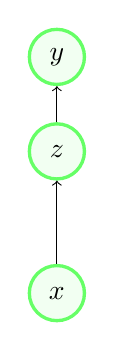
\begin{tikzpicture}[roundnode/.style={circle, draw=green!60, fill=green!5, very thick, minimum size=7mm}]
\node[roundnode] (y) at (0, 0) {$y$};
\node[roundnode] (z) at (0, -1.2) {$z$};
\node[roundnode] (x) at (0, -3) {$x$};
\draw[->] (x) edge (z);
\draw[->] (z) edge (y);
\end{tikzpicture} \hspace{2.5cm} 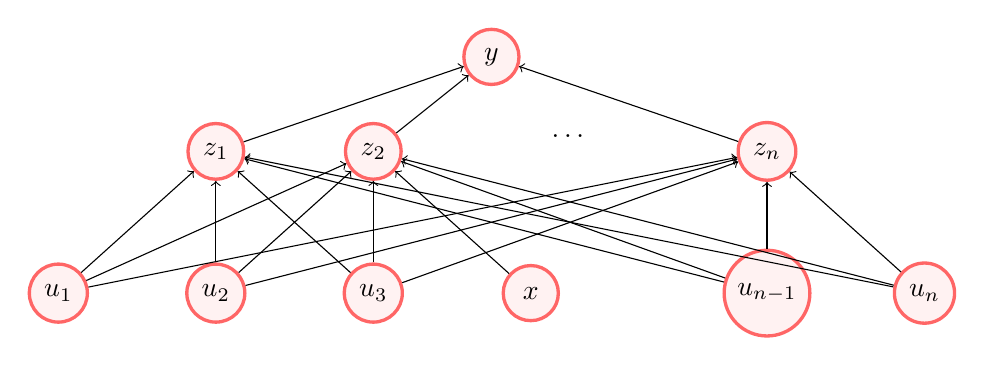
\begin{tikzpicture}[roundnode/.style={circle, draw=red!60, fill=red!5, very thick, minimum size=7mm}]
\node[roundnode] (y) at (1.5, 0) {$y$};
\node[roundnode] (z1) at (-2, -1.2) {$z_1$};
\node[roundnode] (z2) at (0, -1.2) {$z_2$};
\node[roundnode] (zn) at (5, -1.2) {$z_n$};
\node[roundnode] (x) at (2, -3) {$x$};
\node[roundnode] (extra1) at (0, -3) {$u_3$};
\node[roundnode] (extra2) at (-2, -3) {$u_2$};
\node[roundnode] (extran) at (5, -3) {$u_{n-1}$};
\node[roundnode] (side1) at (-4, -3) {$u_1$};
\node[roundnode] (side2) at (7, -3) {$u_n$};
\node (more) at (2.5, -1) {\dots};
\draw[->] (x) edge (z2);
\draw[->] (z1) edge (y);
\draw[->] (z2) edge (y);
\draw[->] (zn) edge (y);
\draw[->] (extra1) edge (z1);
\draw[->] (extra2) edge (z1);
\draw[->] (extra1) edge (z2);
\draw[->] (extra2) edge (z2);
\draw[->] (extra1) edge (zn);
\draw[->] (extra2) edge (zn);
\draw[->] (extran) edge (z1);
\draw[->] (extran) edge (z2);
\draw[->] (extran) edge (zn);
\draw[->] (side1) edge (z1);
\draw[->] (side1) edge (z2);
\draw[->] (side1) edge (zn);
\draw[->] (side2) edge (z1);
\draw[->] (side2) edge (z2);
\draw[->] (side2) edge (zn);

\end{tikzpicture} $$ 

\newpage
\intermediatesubproblem{Consider the case in (a) but now $n$ is small. Create a third plausible causal model (in addition to the two you created in the last problem) using the same graphical depiction style. Your model has to include $x$ and $y$ but is not limited to only those variables.}\spc{5} 
$$ 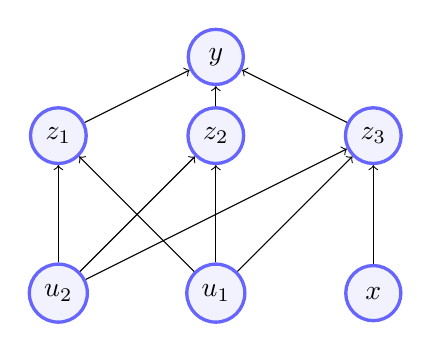
\begin{tikzpicture}[roundnode/.style={circle, draw=blue!60, fill=blue!5, very thick, minimum size=7mm}]
\node[roundnode] (y) at (0, 0) {$y$};
\node[roundnode] (z1) at (-2, -1) {$z_1$};
\node[roundnode] (z2) at (0, -1) {$z_2$};
\node[roundnode] (z3) at (2, -1) {$z_3$};
\node[roundnode] (x) at (2, -3) {$x$};
\node[roundnode] (extra1) at (0, -3) {$u_1$};
\node[roundnode] (extra2) at (-2, -3) {$u_2$};
\draw[->] (x) edge (z3);
\draw[->] (z1) edge (y);
\draw[->] (z2) edge (y);
\draw[->] (z3) edge (y);
\draw[->] (extra1) edge (z1);
\draw[->] (extra2) edge (z1);
\draw[->] (extra1) edge (z2);
\draw[->] (extra2) edge (z2);
\draw[->] (extra1) edge (z3);
\draw[->] (extra2) edge (z3);
\end{tikzpicture} $$ 

\easysubproblem{Explain briefly how you would prove beyond a reasonable doubt that $\x$ is not only correlated with $\y$ but that $\x$ is a causal factor of $\y$.}\spc{3}
\\ 
To prove that $\x$ is a causal factor of $\y$, perform randomized controlled experiments. 

\easysubproblem{Consider $\x$ is college GPA and $\y$ is career average income. Is $\x$ correlated with $\y$? }\spc{3} \\
If $\x$ is college GPA and $\y$ is career average income, then $\x$ is correlated with $\y$. 

\intermediatesubproblem{Consider $\x$ is college GPA and $\y$ is career average income. Is $\x$ a causal factor of $\y$? }\spc{3} \\
If $\x$ is college GPA and $\y$ is career average income, then $\x$ is not a causal factor of $\y$. 

\intermediatesubproblem{Consider $\x$ is college GPA and $\y$ is career average income. Can you think of a $\z$ which is a lurking variable? Explain the variable and why you believe it fits the description of a lurking variable.}\spc{3} \\
If $\x$ is college GPA and $\y$ is career average income, then $z$, a lurking variable, can be the location of career. Different locations can have different career average income. Furthermore, college GPA will come into play when determining whether employers in the location will consider the student for the workforce. 

\intermediatesubproblem{If you fit a linear model for $\y$, $g = b_0 + b_x x + b_z z$, what would the $b_x$ value be close to? Why?}\spc{3} \\
If a linear model for $\y$ is fitted, then the $b_x$ value would be close to $0$.  This is because when $z$ is held constant, the only causal factor in $\y$, manipulating $x$ won't affect $y$ and so $b_x$ would be close to $0$. 

\extracreditsubproblem{Create a causal model using the same graphical depiction style that justifies the four linear regression assumptions. Do so on a different page.}\spc{-0.6}

\newpage
\intermediatesubproblem{When running a regression of \texttt{price} on all variables in the \texttt{diamonds} dataset, the coefficient for \texttt{carat} is about \$6,500. Interpret this value as best as you can.}\spc{4} \\ 
When comparing two observations, A and B, sampled in the same way as the data in \texttt{diamonds}, where A has a \texttt{carat} value one unit higher than the \texttt{carat} value of B, and all other features are exactly the same, then A is predicted to have a response $\texttt{price}_A$ that differs by $\$6,500$, on average, from $\texttt{price}_B$ assuming the linear model optimal for least squares. 

\intermediatesubproblem{When running a logistic regression of class \texttt{malignant} on all variables in the \texttt{biopsy} dataset, the coefficient for \texttt{V1} (which measures clump thickness) is about 0.54. Interpret this value as best as you can.}\spc{5} \\
When comparing two observations, A and B, sampled in the same way as the data in \texttt{biopsy}, where A has a \texttt{V1} value one unit higher than the \texttt{V1} value of B, and all other features are exactly the same, then A is predicted to have a response $\texttt{malignant}_A$ that differs by $0.54$, on average, from $\texttt{malignant}_B$ assuming the logistic model optimal for least squares. 

\end{enumerate}

\problem{Extra Credit Problems} 
\begin{enumerate} 
\extracreditsubproblem{We will now maximize this likelihood w.r.t to $\w$ to find $\b$, the best fitting solution which will be used within $g_{pr}$ i.e.

\beqn
\b = \argmax_{\w \in \reals^{p+1}}\braces{\sum_{i=1}^n \natlog{1 + e^{(1 - 2y_i) \w \cdot \x_i}}}
\eeqn

to do so, we should find the derivative and set it equal to zero i.e.

\beqn
\derivop{\w}{\sum_{i=1}^n \natlog{1 + e^{(1 - 2y_i) \w \cdot \x_i}}} ~\buildrel \text{set} \over =~ 0
\eeqn
}

$$ \begin{aligned} 
\frac{d}{d\w} ( \sum_{i=1}^n \ln (1 + e^{(1-2y_i)\w \cdot \x_i})) &= \sum_{i=1}^n \frac{d}{d\w} \ln (1 + e^{(1-2y_i)\w \cdot \x_i}) \\ &= \sum_{i=1}^n \frac{1}{1 + e^{(1-2y_i)\w \cdot \x_i}} \cdot e^{(1-2y_i)\w \cdot \x_i} \cdot (1-2y_i)\x_i \\ &= \sum_{i=1}^n \frac{(1-2y_i)\x_ie^{(1-2y_i)\w \cdot \x_i}}{1 + e^{(1-2y_i)\w \cdot \x_i}} \\ &= \sum_{i=1}^n (1-2y_i)\x_i \Phi((1-2y_i)\w \cdot \x_i) \end{aligned} $$ 
where $\Phi(u) = \frac{e^u}{1 + e^u}$, the logistic function. Note that there is no closed form for this when set equal to $0$. 

\extracreditsubproblem{Rederive the bias-variance decomposition formula for the average MSE over the distribution $\prob{\X}$ for $y = g + (h^* - g) + (f - h^*) + \delta$. You should group the final expression into \emph{four} terms where two will be the same as the expression found in (c), one will be similar to a term found in (c) and one will be new. Make sure you explain conceptually each term in English. Do so on an additional page.}\spc{-0.5} \\
Here, $Y ~|~ \X = \x = g(\x) + (h^*(\x) - g(\x)) + (f(\x) - h^*(\x)) + \Delta$. Then $$ \expe{(Y - g(\x) | \X)^2} = \expe{(h^*(\x) - g(\x)) + (f(\x - h^*(\x)) + \Delta)^2} $$ Now $$ \begin{aligned} MSE &= \expe{\underbrace{(h^* - g)^2}_{V} + (\underbrace{f-h^*}^B)^2 + \Delta^2 + 2(\underbrace{h^*-g}_{V})\Delta + 2(\underbrace{f-h^*}_{B})\Delta + 2(\underbrace{h^*-g}_{V})(\underbrace{f-h^*}_{B})} 
\\ &= \expe{V^2} + \expe{B^2} + \expe{\Delta^2} + 2\expe{V}\Delta + 2\expe{B\Delta} + 2\expe{VB}
 \\ &= \expe{V^2} + B^2 + \sigma^2 + 2B\expe{V} \end{aligned} $$ 
The $\sigma^2$ term is the variance of $Y$. The $B^2$ term is the bias term, explaining how far $f$ is from the true phenomenon $h^*$. The $\expe{V^2}$ term explains how much $g$ varies from the its mean function $\expe{(h^*-g)^2}$. 

\end{enumerate}

\end{document}








































\problem{These are questions about Silver's book, chapters ...  For all parts in this question, answer using notation from class (i.e. $t ,f, g, h^*, \delta, \epsilon, e, t, z_1, \ldots, z_t, \mathbb{D}, \mathcal{H}, \mathcal{A}, \mathcal{X}, \mathcal{Y}, X, y, n, p, x_{\cdot 1}, \ldots, x_{\cdot p}$, $x_{1 \cdot}, \ldots, x_{n \cdot}$, etc. and also we now have $f_{pr}, h^*_{pr}, g_{pr}, p_{th}$, etc from probabilistic classification as well as different types of validation schemes). }

\begin{enumerate}

\easysubproblem{What algorithm that we studied in class is PECOTA most similar to?}\spc{1}

\easysubproblem{Is baseball performance as a function of age a linear model? Discuss.}\spc{2}

\intermediatesubproblem{How can baseball scouts do better than a prediction system like PECOTA?}\spc{4}

\intermediatesubproblem{Why hasn't anyone (at the time of the writing of Silver's book) taken advantage of Pitch f/x data to predict future success?}\spc{4}

\hardsubproblem{Chapter 4 is all about predicting weather. Broadly speaking, what is the problem with weather predictions? Make sure you use the framework and notation from class. This is not an easy question and we will discuss in class. Do your best.}\spc{6}

\easysubproblem{Why does the weatherman lie about the chance of rain? And where should you go if you want honest forecasts?}\spc{2}

\hardsubproblem{Chapter 5 is all about predicting earthquakes. Broadly speaking, what is the problem with earthquake predictions? It is \textit{not} the same as the problem of predicting weather. Read page 162 a few times. Make sure you use the framework and notation from class.}\spc{6}

\easysubproblem{Silver has quite a whimsical explanation of overfitting on page 163 but it is really educational! What is the nonsense predictor in the model he describes?}\spc{2}


\easysubproblem{John von Neumann was credited with saying that \qu{with four parameters I can fit an elephant and with five I can make him wiggle his trunk}. What did he mean by that and what is the message to you, the budding data scientist? }\spc{5}

\hardsubproblem{Chapter 6 is all about predicting unemployment, an index of macroeconomic performance of a country. Broadly speaking, what is the problem with unemployment predictions? It is \textit{not} the same as the problem of predicting weather or earthquakes. Make sure you use the framework and notation from class.}\spc{6}

\extracreditsubproblem{Many times in this chapter Silver says something on the order of \qu{you need to have theories about how things function in order to make good predictions.} Do you agree? Discuss.}\spc{4}


\end{enumerate}


\problem{This question is about validation for the supervised learning problem with one fixed $\mathbb{D}$.}


\begin{enumerate}

\easysubproblem{For one fixed $\mathcal{H}$ and $\mathcal{A}$ (i.e. one model), write below the steps to do a simple validation and include the final step which is shipping the final $g$.}\spc{6}

\easysubproblem{For one fixed $\mathcal{H}$ and $\mathcal{A}$ (i.e. one model), write below the steps to do a $K$-fold cross validation and include the final step which is shipping the final $g$.}\spc{10}

\intermediatesubproblem{For one fixed $\mathcal{H}$ and $\mathcal{A}$ (i.e. one model), write below the steps to do a bootstrap validation and include the final step which is shipping the final $g$.}\spc{10}

\intermediatesubproblem{For one fixed $\mathcal{H}_1, \ldots \mathcal{H}_M$ and $\mathcal{A}$ (i.e. $M$ different models), write below the steps to do a simple validation and include the final step which is shipping the final $g$.}\spc{22}

\hardsubproblem{For one fixed $\mathcal{H}_1, \ldots \mathcal{H}_M$ and $\mathcal{A}$ (i.e. $M$ different models), write below the steps to do a $K$-fold cross validation and include the final step which is shipping the final $g$. This is not an easy problem! There are a lot of steps and a lot to keep track of...}\spc{22}


\end{enumerate}


\problem{This question is about ridge regression --- an alternative to OLS.}


\begin{enumerate}

\intermediatesubproblem{Imagine we are in the \qu{Luis situation} where we have $\X$ with dimension $n \times (p+1)$ but $p+1 > n$ and we still want to do OLS. Why would the OLS solution we found previously break down in this case?}\spc{4}

\intermediatesubproblem{We will embark now to provide a solution for this case. The solution will also give nice results for other situations besides the Luis situation as well. First, assume $\lambda$ is a positive constant and demonstrate that the expression $\lambda \normsq{\w} = \w^\top (\lambda \I) \w$ i.e. it can be expressed as a quadratic form where $\lambda\I$ is the determining matrix. We will call this term $\lambda \normsq{\w}$ the \qu{ridge penalty}.}\spc{3}


\easysubproblem{Write the $\mathcal{H}$ for OLS below where there parameter is the $\w$ vector. $\w \in$ ?}\spc{1}

\easysubproblem{Write the error objective function that OLS minimizes using vectors, then expand the terms similar to the previous homework assignment.}\spc{1}

\easysubproblem{Now add the ridge penalty $\lambda \normsq{\w}$ to the expanded form you just found and write it below. We will term this two-part error function the \qu{ridge objective}.}\spc{1}

\easysubproblem{Note that the ridge objective looks a bit like the hinge loss we spoke about when we were learning about support vector machines. There are two pieces of this error function in counterbalance. When this is minimized, describe conceptually what is going on.}\spc{5}

\intermediatesubproblem{Now, the ridge penalty term as a quadratic form can be combined with the last term in the least squares error from OLS. Do this, then use the rules of vector derivatives we learned to take $d/d\w$ and write the answer below.}\spc{2}

\easysubproblem{Now set that derivative equal to zero. What matrix needs to be invertible to solve?}\spc{2}

\hardsubproblem{There's a theorem that says \textit{positive definite} matrices are invertible. A matrix is said to be positive definite if every quadratic form is positive for all vectors i.e. if $\forall \z \neq \zerovec~~ \z^\top A \z > 0$ then $A$ is positive definite. Prove this matrix from the previous question is positive definite.}\spc{5}

\easysubproblem{Now that it's positive definite (and thus invertible), solve for the $\w$ that is the argmin of the ridge objective, call it $\b_{ridge}$. Note that this is called the \qu{ridge estimator} and computing it is called \qu{ridge regression} and it was invented by Hoerl and Kennard in 1970.}\spc{3}


\easysubproblem{Did we just figure out a way out of Luis's situation? Explain.}\spc{3}

\intermediatesubproblem{It turns out in the Luis situation, many of the values of the entries of $\b_{ridge}$ are close to 0. Why should that be? Can you explain now conceptually how ridge regression works?}\spc{3}

\easysubproblem{Find $\yhat$ as a function of $\y$ using $\b_{ridge}$. Is $\yhat$ an orthogonal projection of $\y$ onto the column space of $\X$?}\spc{3}

\extracreditsubproblem{Show that this $\yhat$ is an orthogonal projection of $\y$ onto the column space of some matrix $\X_{ridge}$ (which is not $\X$!) and explain how to construct $\X_{ridge}$ on a separate page.}\spc{0}

\easysubproblem{Is the $\mathcal{H}$ for OLS the same as the $\mathcal{H}$ for ridge regression? Yes/no. \\ Is the $\mathcal{A}$ for OLS the same as the $\mathcal{A}$ for ridge regression? Yes/no.}\spc{-0.5}

\intermediatesubproblem{What is a good way to pick the value of $\lambda$, the hyperparameter of the $\mathcal{A}$ = ridge?}\spc{1}




\easysubproblem{In classification via $\mathcal{A}$ = support vector machines with hinge loss, how should we pick the value of $\lambda$? Hint: same as previous question!}\spc{1}



\extracreditsubproblem{Besides the Luis situation, in what other situations will ridge regression save the day?}\spc{3}


\hardsubproblem{The ridge penalty is beautiful because you were able to take the derivative and get an analytical solution. Consider the following algorithm:

\beqn
\b_{lasso} = \argmin_{\w~\in~\reals^{p + 1}} \braces{(\y - \X\w)^\top(\y - \X\w) + \lambda \norm{\w}^1}
\eeqn

This penalty is called the \qu{lasso penalty} and it is different from the ridge penalty in that it is not the norm of $\w$ squared but just the norm of $\w$. It turns out this algorithm (even though it has no closed form analytic solution and must be solved numerically a la the SVM) is very useful! In \qu{lasso regression} the values of $\b_{lasso}$ are not shrunk \textit{towards} 0 they are harshly punished \textit{directly to} 0! How do you think lasso regression would be useful in data science? Feel free to look at the Internet and write a few sentences below.}~\spc{6}

\easysubproblem{Is the $\mathcal{H}$ for OLS the same as the $\mathcal{H}$ for lasso regression? Yes/no. \\ Is the $\mathcal{A}$ for OLS the same as the $\mathcal{A}$ for lasso regression? Yes/no.}\spc{-0.5}

\end{enumerate}

\problem{These are questions about non-parametric regression.}


\begin{enumerate}

\easysubproblem{In problem 1, we talked about schemes to validate algorithms which tried $M$ different prespecified models. Where did these models come from?}\spc{4}

\intermediatesubproblem{What is the weakness in using $M$ pre-specified models?}\spc{5}

\hardsubproblem{Explain the steps clearly in forward stepwise linear regression.}\spc{6}

\hardsubproblem{Explain the steps clearly in \emph{backwards} stepwise linear regression.}\spc{7}

\intermediatesubproblem{What is the weakness(es) in this stepwise procedure?}\spc{4}

\easysubproblem{Define \qu{non-parametric regression}. What problem(s) does it solve? What are its goals? Discuss.}\spc{7}

\intermediatesubproblem{Provide the steps for the regression tree (the one algorithm we discussed in class) below.}\spc{10}


\easysubproblem{Consider the following data 

\begin{figure}[htp]
\centering
\includegraphics[width=3in]{curvy}
\end{figure}

Create a tree with maximum depth 1 (i.e one split at the root node) and plot $g$ above.}~\spc{4}


\easysubproblem{Now add a second split to the tree and plot $g$ below.

\begin{figure}[htp]
\centering
\includegraphics[width=3in]{curvy}
\end{figure}

}~\spc{-0.5}


\easysubproblem{Now add a third split to the tree and plot $g$ below.

\begin{figure}[htp]
\centering
\includegraphics[width=3in]{curvy}
\end{figure}

}~\spc{5}


\easysubproblem{Now add a fourth split to the tree and plot $g$ below.

\begin{figure}[htp]
\centering
\includegraphics[width=3in]{curvy}
\end{figure}

}~\spc{-0.5}

\easysubproblem{Draw a tree diagram of $g$ below indicating which nodes are the root, inner nodes and leaves. Indicate split rules and leaf values clearly.}\spc{15}



\easysubproblem{Plot $g$ below for the mature tree with the default $N_0 =$ \texttt{nodesize} hyperparameter.

\begin{figure}[htp]
\centering
\includegraphics[width=3in]{curvy}
\end{figure}

}~\spc{-0.5}


\easysubproblem{If $N_0 =1$, what would likely go wrong?}\spc{2}

\easysubproblem{How should you pick the $N_0 =$ \texttt{nodesize} hyperparameter in practice?}\spc{2}


\end{enumerate}


\problem{These are questions about classification trees.}


\begin{enumerate}

\easysubproblem{How are classification trees different than regression trees?}\spc{2}

\intermediatesubproblem{What are the steps in the classification tree algorithm?}\spc{12}


\end{enumerate}

\problem{These are questions about measuring performance of a classifier.}

\begin{enumerate}

\easysubproblem{What is a confusion table?}\spc{8}


Consider the following in-sample confusion table where \qu{$>50$K} is the positive class:

\begin{Verbatim}
       y_hats_train
y_train <=50K >50K
  <=50K  3475  262
  >50K    471  792
\end{Verbatim}

\easysubproblem{Calculate the following: $n$ (sample size) = \\~\\
$FP$ (false positives) = \\~\\
$TP$ (true positives) = \\~\\
$FN$ (false negatives) = \\~\\
$TN$ (true negatives) = \\~\\
$\#P$ (number positive) = \\~\\
$\#N$ (number negative) = \\~\\
$\#PP$ (number predicted positive) = \\~\\
$\#PN$ (number predicted negative) = \\~\\
$\#P / n$ (prevalence / marginal rate / base rate) = \\~\\
$(FP + FN) / n$ (misclassification error) = \\~\\
$(TP + TN) / n$ (accuracy) = \\~\\
$TP / \#PP$ (precision) = \\~\\
$TP / \#P$ (recall, sensitivity, true positive rate, TPR) = \\~\\
$2 / (\text{recall}^{-1} + \text{precision}^{-1})$ (F1 score) = \\~\\
$FP / \#PP$ (false discovery rate, FDR) = \\~\\
$FP / \#N$ (false positive rate, FPR) = \\~\\ %false alarm rate 
$FN / \#PN$ (false omission rate, FOR) = \\~\\
$FN / \#P$ (false negative rate, FNR) = %miss rate 
}

\easysubproblem{Why is FPR also called the \qu{false alarm rate}?}\spc{4}

\easysubproblem{Why is FNR also called the \qu{miss rate}?}\spc{4}


\easysubproblem{Below let the red icons be the positive class and the blue icons be the negative class. 


\begin{figure}[htp]
\centering
\includegraphics[width=1.5in]{precision_recall.jpg}
\end{figure}

The icons included inside the black border are those that have $\hat{y} = 1$. Compute both precision and recall.}\spc{4}

\intermediatesubproblem{There is always a tradeoff of FP vs FN. However, in some situations, you will look at FPR vs. FNR. Describe such a classification scenario. It does not have to be this income amount classification problem, it can be any problem you can think of.}\spc{3}

\intermediatesubproblem{There is always a tradeoff of FP vs FN. However, in some situations, you will look at FDR vs. FOR. Describe such a classification scenario. It does not have to be this income amount classification problem, it can be any problem you can think of.}\spc{3}

\intermediatesubproblem{There is always a tradeoff of FP vs FN. However, in some situations, you will look at precision vs. recall. Describe such a classification scenario. It does not have to be this income amount classification problem, it can be any problem you can think of.}\spc{3}


\intermediatesubproblem{There is always a tradeoff of FP vs FN. However, in some situations, you will look only at an overall metric such as accuracy (or $F1$). Describe such a classification scenario. It does not have to be this income amount classification problem, it can be any problem you can think of.}\spc{4}

\end{enumerate}







\end{document}

\problem{These are questions about Silver's book, chapter 2.}


\begin{enumerate}

\intermediatesubproblem{If one's goal is to fit a model for a phenomenon $y$, what is the difference between the approaches of the hedgehog and the fox? Answer using notation from class (i.e. $t ,f, g, h^*, \delta, \epsilon, e, t, z_1, \ldots, z_t, \mathbb{D}, \mathcal{H}, \mathcal{A}, \mathcal{X}, \mathcal{Y}, X, y, n, p, x_{\cdot 1}, \ldots, x_{\cdot p}, x_{1 \cdot}, \ldots, x_{n \cdot}$, etc.). Connecting this to the modeling framework should really make you think about what Tetlock's observation means for political and historical phenomena.}\spc{4}

\easysubproblem{Why did Harry Truman like hedgehogs? Are there a lot of people that think this way?}\spc{4}


\hardsubproblem{Why is it that the more education one acquires, the less accurate one's predictions become?}\spc{4}


\easysubproblem{Why are probabilistic classifiers (i.e. algorithms that output functions that return probabilities) better than vanilla classifiers (i.e. algorithms that only return the class label)? We will move in this direction in class soon.}\spc{4}

\end{enumerate}

\problem{These are questions about Finlay's book, chapter 2-4. We will hold off on chapter 1 until we cover probability estimation after midterm 2.}


\begin{enumerate}

\easysubproblem{What term did we use in class for \qu{behavioral (outome) data}?}\spc{0}

\easysubproblem{Write about some reasons why data scientists implement models that are subpar in predictive performance (p27).}\spc{3}


\easysubproblem{In the first wine example, what is the outcome metric and what kind of supervised learning was employed?}\spc{0}

\easysubproblem{In the second wine example, what is the outcome metric and kind of supervised learning was employed?}\spc{0}


\easysubproblem{In the third chapter, why is it that some organizations cannot use predictive modeling to improve their business?}\spc{3}

\easysubproblem{In the bankruptcy case, what is the problem with merely using $g$ to obtain a $\hat{y}$ without any other information from the model?}\spc{3}

\easysubproblem{Chapter 3 talks about using the model with human judgment. Under what circumstances is this beneficial? Answer using notation from class (i.e. $t ,f, g, h^*, \delta, \epsilon, e, t$, $z_1, \ldots, z_t, \mathbb{D}, \mathcal{H}, \mathcal{A}, \mathcal{X}, \mathcal{Y}, X, y, n, p, x_{\cdot 1}, \ldots, x_{\cdot p}, x_{1 \cdot}, \ldots, x_{n \cdot}$, etc.).}\spc{3}


\hardsubproblem{In Chapter 4 Finaly makes an interesting observation based on his experience in data science. He says most predictive models have $p \leq 30$. Why do you think this is? Discuss.}\spc{5}


\easysubproblem{He says there is \qu{almost always other data that could be acquired ... [which] doesn't always come for free}. The \qu{data} he is talking about here specifically means \qu{more predictors} i.e. increasing $p$. In what cases would someone be willing to pay for this data?}\spc{3}


\easysubproblem{Table 4 lists \qu{data types} about what type of observations?}\spc{1}

\easysubproblem{What type of data does he find in his experience to be the most important to predictive modeling? Why do you think this is so?}\spc{3}

\easysubproblem{If $x_{\cdot 17}$ was age and $x_{\cdot 18}$ is age of spouse, what is the most likely reason why adding $x_{\cdot 18}$ to $\mathbb{D}$ not be friutful for predictive ability?}\spc{3}

\hardsubproblem{What is the lifespan of a predictive model? Why does it not last forever? Answer using notation from class (i.e. $t ,f, g, h^*, \delta, \epsilon, e, t$, $z_1, \ldots, z_t, \mathbb{D}, \mathcal{H}, \mathcal{A}, \mathcal{X}, \mathcal{Y}, X, y, n, p$, $x_{\cdot 1}, \ldots, x_{\cdot p}, x_{1 \cdot}, \ldots, x_{n \cdot}$, etc.).}\spc{3}


\hardsubproblem{What does \qu{large enough to representative of the full population} (p80) mean? Answer using notation from class (i.e. $t ,f, g, h^*, \delta, \epsilon, e, t$, $z_1, \ldots, z_t, \mathbb{D}, \mathcal{H}, \mathcal{A}, \mathcal{X}, \mathcal{Y}, X, y, n, p$, $x_{\cdot 1}, \ldots, x_{\cdot p}, x_{1 \cdot}, \ldots, x_{n \cdot}$, etc.).}\spc{3}

\easysubproblem{Is there a hype about \qu{big data} i.e. including millions of observations instead of a few thousand? Discuss Finlay's opinion.}\spc{3}


\easysubproblem{What is Finlay's solution to \qu{overfitting} (p84)?}\spc{5}
\end{enumerate}


\problem{These are questions about association and correlation.}


\begin{enumerate}

\easysubproblem{Give an example of two variables that are both correlated and associated by drawing a plot.}\spc{4}

\easysubproblem{Give an example of two variables that are not correlated but are associated by drawing a plot.}\spc{4}

\easysubproblem{Give an example of two variables that are not correlated nor associated by drawing a plot.}\spc{4}

\easysubproblem{Can two variables be correlated but not associated? Explain.}\spc{4}


\end{enumerate}

\problem{These are questions about multivariate linear model fitting using the least squares algorithm.}

\begin{enumerate}

\hardsubproblem{Derive $\partialop{\c}{\c^\top A \c}$ where $\c \in \reals^n$ and $A \in \reals^{n \times n}$ but \textit{not} symmetric. Get as far as you can.}\spc{8}

\easysubproblem{Given matrix $X \in \reals^{n \times (p+1)}$, full rank and first column consisting of the $\onevec_n$ vector, rederive the least squares solution $\b$ (the vector of coefficients in the linear model shipped in the prediction function $g$). No need to rederive the facts about vector derivatives.}\spc{10}

\intermediatesubproblem{Consider the case where $p = 1$. Show that the solution for $\b$ you just derived is the same solution that we proved for simple regression in Lecture 8. That is, the first element of $\b$ is the same as $b_0 = \ybar - r \frac{s_y}{s_x}\xbar$ and the second element of $\b$ is $b_1 = r \frac{s_y}{s_x}$.} \spc{10}

\easysubproblem{If $X$ is rank deficient, how can you solve for $\b$? Explain in English.} \spc{2}

\hardsubproblem{Prove $\rank{X} =\rank{X^\top X}$.}\spc{6}

\hardsubproblem{Given matrix $X \in \reals^{n \times (p+1)}$, full rank and first column consisting of the $\onevec_n$ vector, now consider cost multiples (\qu{weights}) $c_1, c_2, \ldots, c_n$ for each mistake $e_i$. As an example, previously the mistake for the 17th observation was $e_{17} := y_{17} - \hat{y}_{17}$ but now it would be $e_{17} := c_{17} (y_{17} - \hat{y}_{17})$.  Derive the weighted least squares solution $\b$. No need to rederive the facts about vector derivatives. Hints: (1) show that SSE is a quadratic form with the matrix $C$ in the middle (2) Split this matrix up into two pieces i.e. $C = C^{\half} C^{\half}$, distribute and then foil (3) note that a scalar value equals its own transpose and (4) use the vector derivative formulas.}\spc{20}


\hardsubproblem{If $p=1$, prove $r^2 = R^2$ i.e. the linear correlation is the same as proportion of sample variance explained in a least squares linear model.}\spc{6}


\intermediatesubproblem{Prove that the point $<1,\xbar_1, \xbar_2, \ldots, \xbar_p, \bar{y}>$ is a point on the least squares linear solution.}\spc{13}

\end{enumerate}

\problem{These are questions related to the concept of orthogonal projection, QR decomposition and its relationship with least squares linear modeling.}

\begin{enumerate}

\easysubproblem{Consider least squares linear regression using a design matrix $X$ with rank $p + 1$. What are the degrees of freedom in the resulting model? What does this mean?}\spc{3}


\intermediatesubproblem{If you are orthogonally projecting the vector $\y$ onto the column space of $X$ which is of rank $p + 1$, derive the formula for $\proj{\colsp{X}}{\y}$. Is this the same as the least squares solution?}\spc{6}

\hardsubproblem{We saw that the perceptron is an \textit{iterative algorithm}. This means that it goes through multiple iterations in order to converge to a closer and closer $\w$. Why not do the same with linear least squares regression? Consider the following. Regress $\y$ using $\X$ to get $\yhat$. This generates residuals $\e$ (the leftover piece of $\y$ that wasn't explained by the regression's fit, $\yhat$). Now try again! Regress $\e$ using $\X$ and then get new residuals $\e_{new}$. Would $\e_{new}$ be closer to $\zerovec_n$ than the first $\e$? That is, wouldn't this yield a better model on iteration \#2? Yes/no and explain.}\spc{10}


\intermediatesubproblem{Prove that $Q^\top = Q^{-1}$ where $Q$ is an orthonormal matrix such that $\colsp{Q} = \colsp{X}$ and $Q$ and $X$ are both matrices $\in \reals^{n \times (p+1)}$. Hint: this is purely a linear algebra exercise.}\spc{10}


\intermediatesubproblem{Prove that the least squares projection $H = \XXtXinvXt$ is the same as $QQ^\top$.}\spc{10}

\intermediatesubproblem{Prove that an orthogonal projection onto the $\colsp{Q}$ is the same as the sum of the projections onto each column of $Q$.}\spc{10}


\hardsubproblem{Trouble in paradise. Prove that the SSE of a multivariate linear least squares model always decreases (equivalently, $R^2$ always increases) upon the addition of a new independent predictor. Keep in mind this holds true even if this new predictor has no information about the true causal inputs to the phenomenon $y$.}\spc{12}

\intermediatesubproblem{Why is this a bad thing? Explain in English.}\spc{3}



\extracreditsubproblem{Prove that $\rank{H} =\tr{H}$.}\spc{-0.5}

\end{enumerate}


\end{document}